%Tex-Stuff
\documentclass[a4paper,12pt]{article}

%Imports
\usepackage[pdftex]{graphicx}
\usepackage[utf8]{inputenc}
\usepackage{subcaption}
\usepackage{hyperref}
%\usepackage{enumitem}


%%%%%%%%%%%%%%%%%%%%%%%%%%%%%%%%%%%%%%%%%%%%%%%%
\begin{document}

\section{PaperOverflow: Produktivision}
Die Beschreibung der Produktvision erfolgt noch den Feldern des  \href{http://www.romanpichler.com/tools/vision-board/}{"Product-Vision-Boards"} von Roman Pichler. 
\begin{figure}[h!]
  \centering
  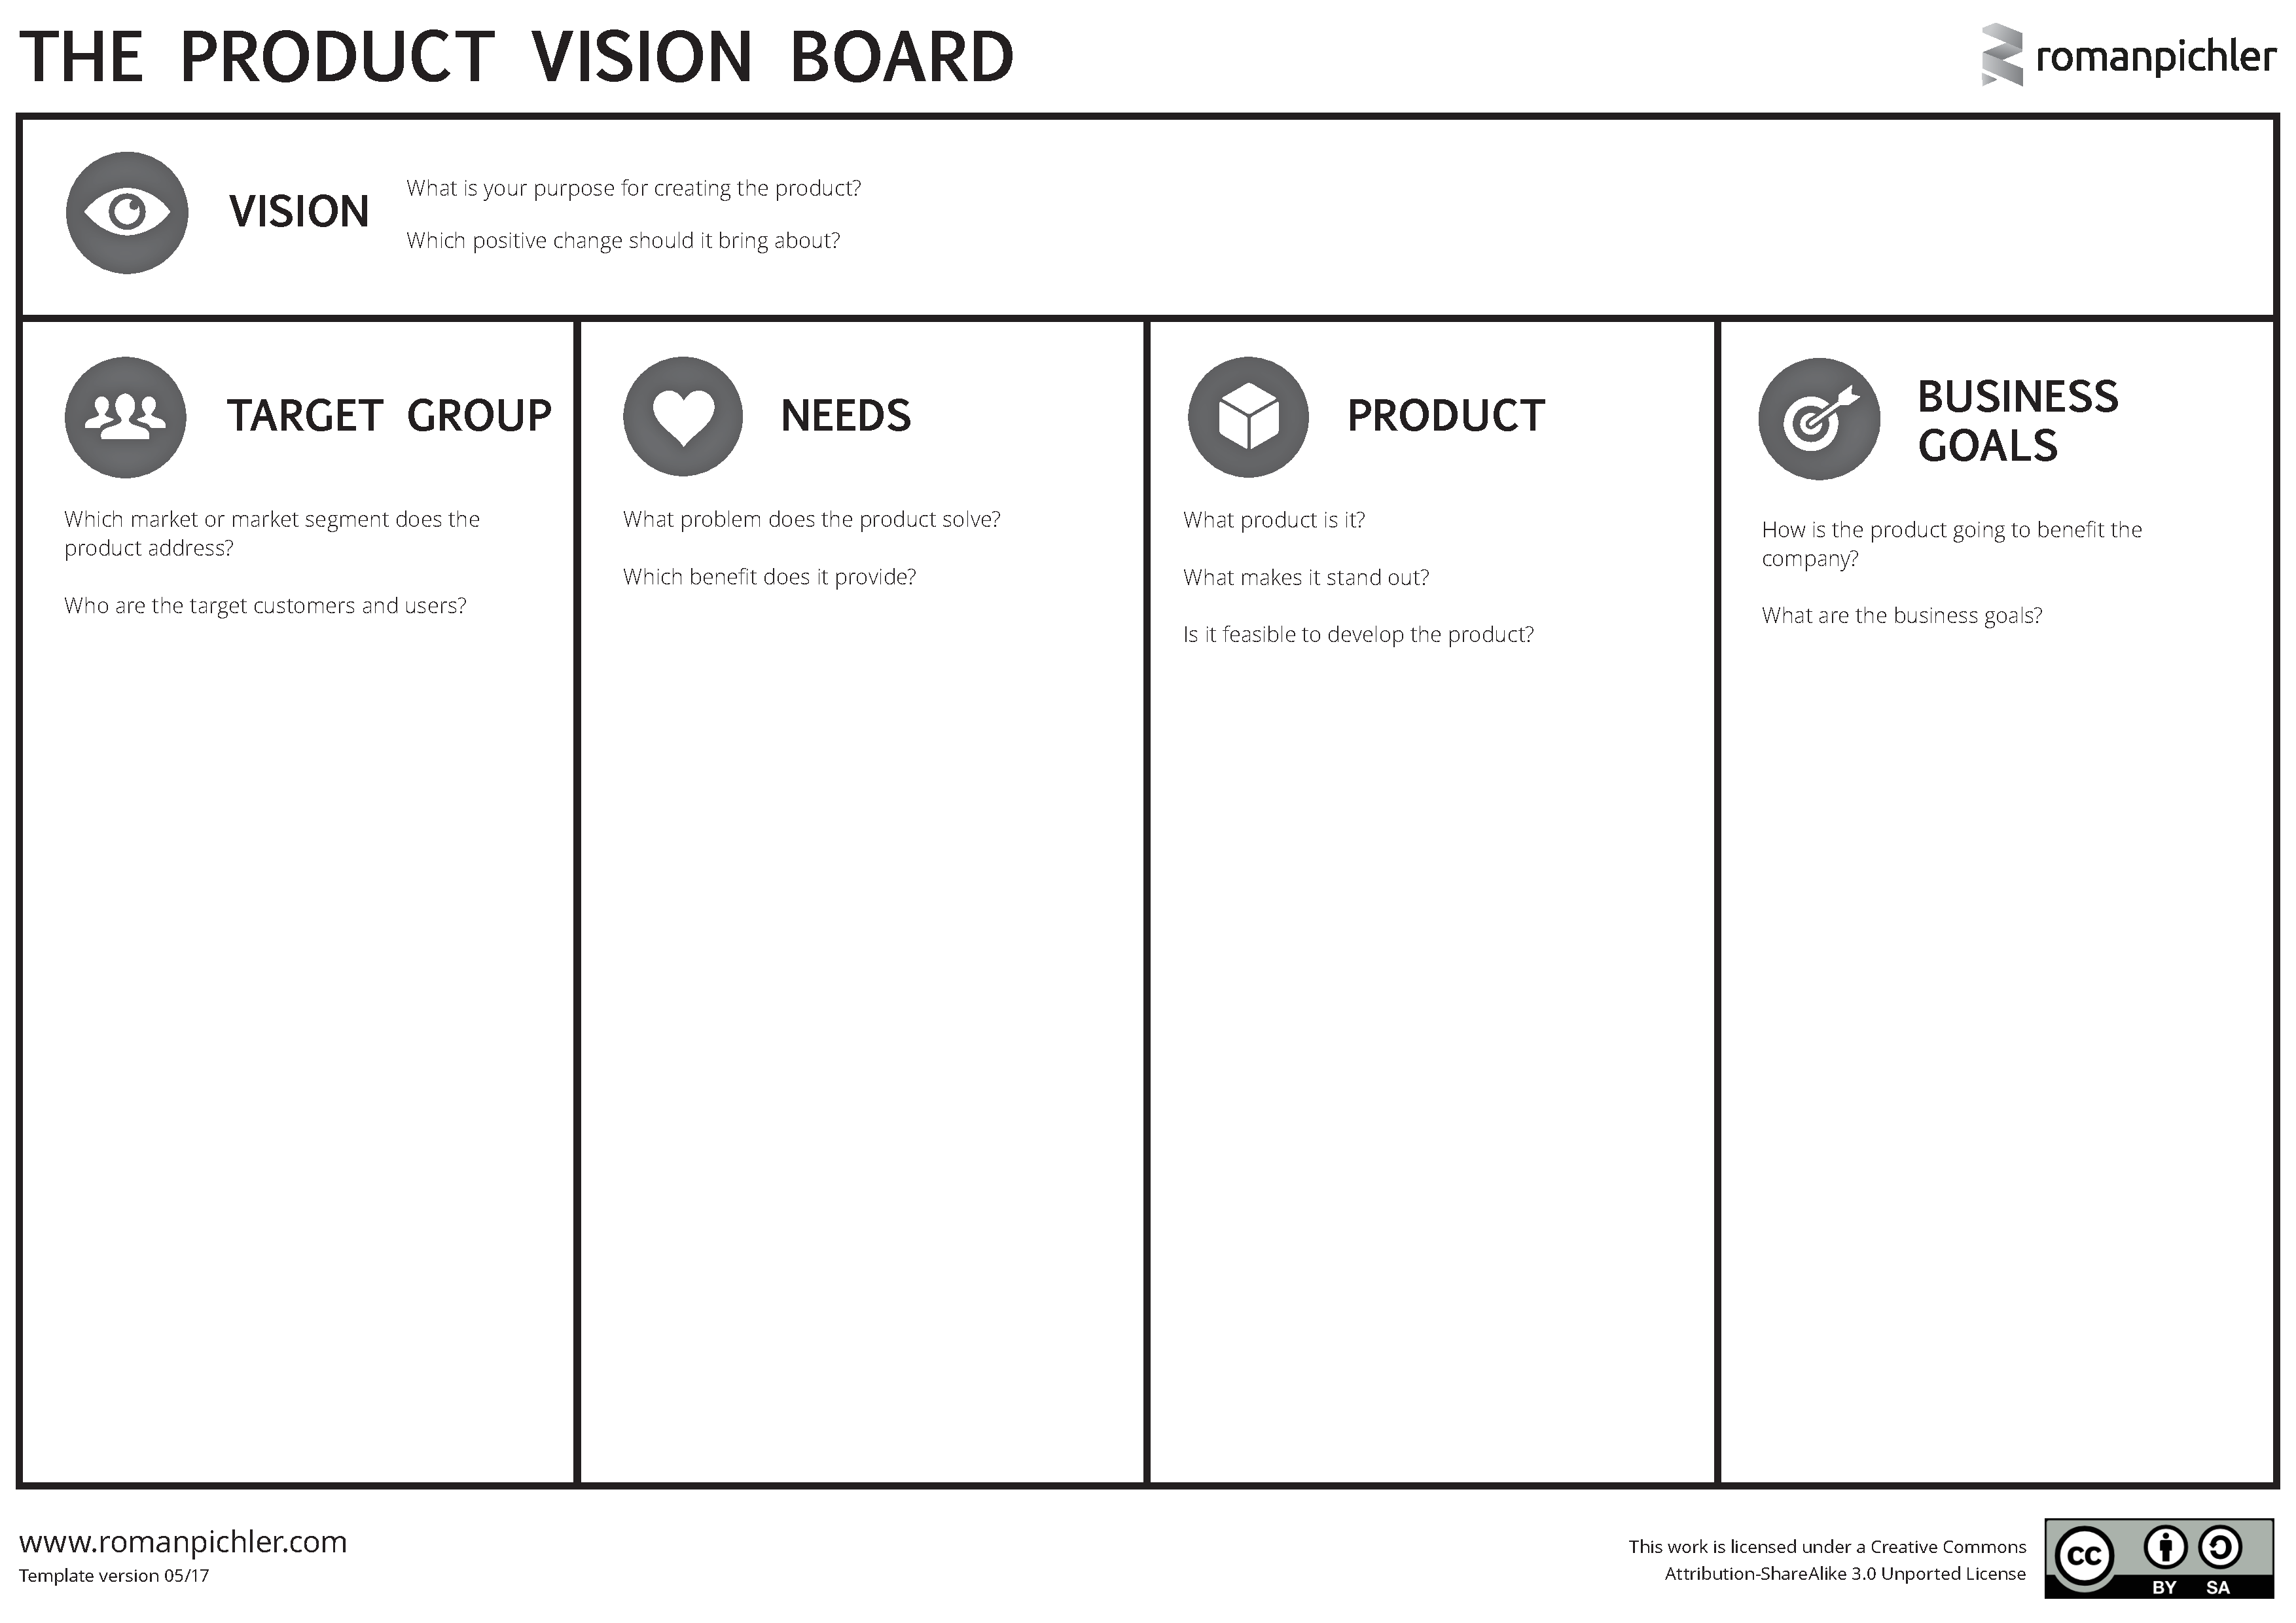
\includegraphics[width=0.7\linewidth]{res/PVB.pdf}
\end{figure}

Besonderes Augenmerk soll dabei auf die Produktbeschreibung gelegt werden.
Die Geschäfts-Ziele hingegen, sollen aufgrund der geringen Relevanz für das Projekt nicht beleuchtet werden.
\subsection{Vision}
\begin{itemize}
\item Das Produkt gibt's im wesentlichen schon in vielen Formen. Es geht nicht darum, dass wir die Funktionen anbieten, sondern dass wir sie \underline{in einer komfortabelen Form} zur Verfügung stellen.
\item Angenehmes und unkompliziertes Arbeiten mit Literatur.
\item Je mehr Literatur desto besser und nicht desto unhandlicher.
\end{itemize}

\subsection{Zielgruppe}
Verfasser wissenschftlicher Texte:
\begin{itemize}
	\item  Anfänger
	\item Fortgeschrittene
	\item Besonders: Viel-Dokumenten-Verfasser
\end{itemize}

\subsection{Bedürfnisse}
\begin{itemize}
\item Komfortables hinzufügen von Literaturquellen
\item Überblick behalten. $\to$ Komfortables verwalten von Literaturquellen
\item Angenehmes Suchen, schnelles finden, Komfort-Funktionen.
\item Zum Zitat in wenigen Klicks.
\item Ordnung über digitale Dokumente behalten.
\item Sicherstellen von Einhaltung der Zitierstandards
\end{itemize}

\subsection{Produktbeschreibung}

Sie haben sich dazu entschieden eine wissenschaftliche Arbeit zu verfassen und sind nun dabei sich Wissen zum Themengebiet heranzuziehen? Und der Haufen der Veröffentlichungen wir immer größer und größer? Und ganz allmählich unbezwingbar? Sie nähern sich langsam der Grenze, ab der sie einfach nicht mehr Dokumente handhaben können? Dem Overflow an Papers? 
\begin{center}
Keine Panik! 
\end{center}
Der Overflow ist nicht böse, er braucht nur die richtige Handhabe. Mit PaperOverflow holen Sie das Maximum aus Ihrer Dokumentensammlung heraus!\\ \\
PaperOverflow unterstützt Sie in Ihrem Arbeiten, in den drei folgenden Schritten:

\renewcommand\thesubfigure{\thefigure}
\begin{figure}[h!]
  \centering
  \begin{subfigure}[b]{0.32\linewidth}
    
\includegraphics[width=\linewidth]{res/step1.png}
    \caption{Den PaperOverflow nähren.}
  \end{subfigure}
  \begin{subfigure}[b]{0.32\linewidth}
    
\includegraphics[width=\linewidth]{res/step2.png}
    \caption{Den PaperOverflow durchsuchen}
  \end{subfigure}
  \begin{subfigure}[b]{0.32\linewidth}
    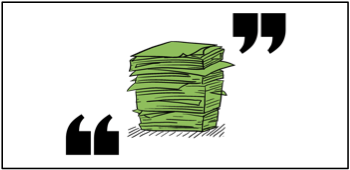
\includegraphics[width=\linewidth]{res/step3.png}
    \caption{Den PaperOverflow zitieren}
  \end{subfigure}
\end{figure}



\paragraph{Nähern Sie den PaperOverflow}
PaperOverflow unterstützt Sie bei der Verwaltung Ihrer Dokumente. Diese legt PaperOverflow für Sie ab und ergänzt die Meta-Informationen, die Sie für das Durchsuchen und Zitieren benötigen.

\paragraph{Arbeiten Sie mit dem PaperOverflow}
PaperOverflow stellt Ihnen nützliche Funktionalitäten für das Durchsuchen ihres gesammelten Overflows zur Verfügung. Suchen Sie nach Autoren, Stichworten und erhalten Sie Vorschläge für ähnliche Dokumente. Dank dieser Funktionen wird die Trefferquote für ein gelungenes Zitat umso höher, je mehr Papers ihr Overflow 

\paragraph{Zitieren Sie den PaperOverflow}
passende Zitat in Ihrem Overflow gefunden? Zitieren Sie! Mit einem Klick haben Sie den entsprechenden BibTex in der Zwischenablage und können Ihn weiterverarbeiten. Sie möchten zunächst weiter nach Zitierbaren Stellen suchen? Legen Sie sich eine Zitat-Sammlungen an und exportieren Sie diese!

%\pagebreak

\end{document}
%%%%%%%%%%%%%%%%%%%%%%%%%%%%%%%%%%%%%%%%%%%%%%%%